% !TEX TS-program = xelatex
% !TEX encoding = UTF-8

% Delta, marzec 1991
%
% Tekst i rysunki:
% http://deltami.edu.pl/temat/matematyka/analiza/2011/03/26/Czy_krowe_mozna_wpisac_w_kwadrat/
%
% Tytuł: Czy krowę można wpisac w kwadrat?
% Autorzy: Krzysztof Ciesielski i Zdzisław Pogoda

\documentclass[a4paper,12pt]{article}

% ftp://sunsite.icm.edu.pl/pub/CTAN/macros/latex/contrib/unicode-math/unicode-math.pdf
% http://www.charlietanksley.net/philtex/the-unicode-math-package-for-xelatex-and-the-stix-fonts/
\usepackage{fontspec,xunicode,unicode-math}

\defaultfontfeatures{Ligatures=TeX,Scale=MatchLowercase}

\setmainfont{Minion Pro}
\setmathfont{xits-math.otf}
%\setmathfont{Asana-Math.otf}
%\setmathfont{lmmath-regular.otf}
%\setmathfont{STIXGeneral}
%\usepackage{mathpazo}

\usepackage{graphicx} % ftp://ftp.tex.ac.uk/tex-archive/info/epslatex.pdf

\usepackage{polyglossia}
\setdefaultlanguage{polish}

\usepackage{wrapfig}

\usepackage[parfill]{parskip} % akapity oddzielamy pustym wierszem

\renewcommand{\labelitemi}{--}

\begin{document}
\pagestyle{empty}

\section*{Czy krowę można wpisać w kwadrat?}

\begin{abstract}
Jednym z najważniejszych pojęć matematycznych jest ciągłość.
Założenie jej prowadzi do bardzo interesujących,
a czasem nawet zaskakujących wniosków.
Klasyczną własnością (zwaną własnością Darboux choć to
nie Gaston Darboux jest jej autorem!)
jest przyjmowanie wszystkich wartości pośrednich przez
funkcję ciągłą na przedziale,oraz uogólnienia tego faktu.
Konsekwencje tego mogą nas niejednokrotnie zaskoczyć.
\end{abstract}

Oto przykład: jakąkolwiek postać (np. krowę lub kota)
narysuje dziecko na kartce, zawsze można ją wpisać w kwadrat.
Bardziej matematycznie: jeśli $K$ jest krzywą zamkniętą 
na płaszczyźnie, to $K$ na zawsze można opisać kwadrat.

\begin{wrapfigure}[12]{l}{4.5cm}
%\vspace{-8pt}
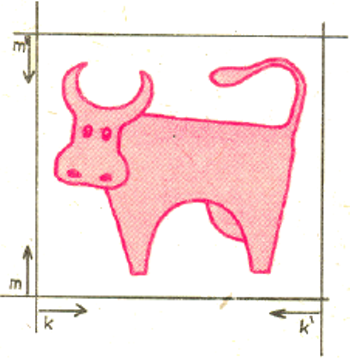
\includegraphics[width=4.5cm]{krowa-1}
%\caption{Krowa}
\vspace{-20pt}
\center{\small\bf Rys. 1}
\label{krowa}
\end{wrapfigure}

Co to znaczy: wpisać krzywą w kwadrat lub – ogólniej – w prostokąt?
Wybierzmy dowolną linię prostą $m$ rozłączną z daną krzywą (Rys.~\ref{krowa}) 
i przesuwajmy ją prostopadle do jej kierunku,
aż do momentu zetknięcia się z krzywą.
Następnie wybieramy taką prostą $m'$ równoległą do $m'$   
że krzywa leży między obiema prostymi i znów przesuwamy ją tak,
by zetknęła się z krzywą. Dalej wybieramy dwie proste $k$
i~$k'$, prostopadłe do $m$ takie, by krzywa była zawarta między nimi,
a następnie powtarzamy operację jak w przypadku
$m$ i~$m'$. Otrzymane proste wyznaczają pewien prostokąt, 
w~który krzywa będzie wpisana.

Krótko mówiąc, krzywa jest wpisana w prostokąt,
gdy się w nim zawiera i z każdym z boków ma przynajmniej
jeden punkt wspólny. Mając dany dowolny kierunek
możemy skonstruować prostokąt, w który krzywa
jest wpisana, i którego jeden z boków wyznacza 
tenże kierunek. Pokażemy, że zawsze można wybrać
kierunek tak, by prostokąt ów był kwadratem. 

\end{document}